\documentclass[onehalfspacing,11pt]{article}
\usepackage{achicago,setspace,palatino,graphicx}
\usepackage{amsmath,amssymb}
\usepackage{bm,bbm}
\usepackage[bottom]{footmisc} % places footnotes @ bottom of page
\usepackage{tabularx,booktabs}
\usepackage{enumerate}
\usepackage[breaklinks]{hyperref} % option enables "broken" links across lines
\usepackage{natbib}
\usepackage[usenames,dvipsnames]{pstricks}
\usepackage{epsfig}
\usepackage{caption}
\usepackage{subcaption}
\usepackage{lscape,rotating}
\usepackage{xfrac}
\usepackage{dsfont}
\usepackage{multicol}
\newtheorem{as}{Assumption}
\newtheorem{conjecture}{Conjecture}
\newtheorem{corr}{Corollary}
\newtheorem{df}{Definition}
\newtheorem{lemma}{Lemma}
\newtheorem{prp}{Proposition}
\newtheorem{clm}{Claim}
\newtheorem{rmk}{Remark}
\newenvironment{prf}{{\bf Proof}}{\hfill {\sc q.e.d. }}
\newenvironment{prfLemma}{{\bf Proof of Lemma}}{\hfill {\sc q.e.d. }(Lemma)}
\setlength{\parindent}{0em}
\setlength{\parskip}{1.5ex plus0.5ex
minus0.5ex} \textwidth15.75cm \evensidemargin5mm \oddsidemargin5mm
\topmargin-8mm \textheight 21.7cm

\newcommand{\fraction}{\int\frac{\mu_{t+1}}{\epsilon_{t+1}} }
\newcommand{\lbar}{\int\frac{\mu_{t+1}}{\epsilon_{t+1}} }
\newcolumntype{Y}{>{\centering\arraybackslash}X}
\parindent 0pt
\parskip 5pt
\def\newblock{\hskip .11em plus .33em minus .07em}
\hypersetup{colorlinks=true,urlcolor=blue,linkcolor=blue,citecolor=blue}

%%%%%%%%%%%%%%%%%%%%%%%%%%%%%%%%%%%%%%%%%%%%%%%%%%%%%%%%%%%%%%%%%%%%%

\begin{document}

\begin{titlepage}
%\begin{singlespacing}

\title{Industry Clusters\footnote{Nicole Jieying Zhang, Zili Yang, and Weihao Lu provided outstanding research assistance.}}

\author{Simeon D.~Alder\footnote{University of Wisconsin - Madison, Department of Economics, email: \url{simeon.alder@wisc.edu}}}
%\date{October 2011}
\date{\today} % \\ \vspace{5mm} {\sc Preliminary and Incomplete}}

\maketitle
%
%\begin{abstract}
%
%\end{abstract}
%\noindent
%\textit{JEL Codes:} 
%
%\textit{Keywords:} 
%\end{singlespacing}
\end{titlepage}

%\begin{onehalfspacing}

\section{Introduction}
The U.S.~economy has been characterized by a continuous reallocation of labor and capital across industries and space. Some of this reallocation is driven by long-term trends while other instances are the result of short-term or temporary shocks.

Long-term structural change has been associated with a secular decline in agricultural employment and steady rise of employment in the service sector, while manufacturing employment exhibits more of a hump-shaped pattern as real incomes per capita rise over time \citep{Herrendorf:2013b}. In the short run, the effects of an event like the COVID-19 pandemic can be very uneven across industries and space. Online retailers like Amazon expanded their workforce significantly with both permanent and temporary workers while bars and restaurants, for instance, were subject to local public health restrictions and employment in the leisure and hospitality industries shrank accordingly. More generally, due to variation in the local industry mix and public health measures, some labor markets experienced more significant disruptions than others and some of these are of a temporary nature while other will have lingering effects.

In recent years, a growing literature has analyzed the effects of various shocks and policies on local employment growth. \cite{Autor:2013}, for instance, find that approximately one quarter of the observed decline in manufacturing employment can be attributed to a surge of light manufactured imports from China between 1990 and 2007. Locally, more exposed Commuting Zones (CZs) in terms of import competition experienced larger labor market disruptions.\footnote{Commuting Zones are delineations of local labor markets without regard for administrative boundaries like county or state lines. They are based on journey-to-work data and define clusters of counties with strong commuting ties. The commuting zone is the lowest level of geography for local labor markets and does not depend on population size.} \cite{Fort:2018} find that trade and technological innovation both contribute to declining manufacturing employment. In contrast to \cite{Autor:2013}, they analyze {\it national} employment at the 3-digit NAICS subsector level. Local variation in the impact of industry-level shocks is due to variations in the local industry concentration. They also emphasize that, empirically, a trade vs. technology decomposition of the decline is rather challenging.\footnote{A 2017 Wall Street Journal article with the title ``Foreign Robots Invade American Factory Floors'' about {\it Marlin Steel Wire Products LLC} illustrates the challenge \citep{Michaels:2017}.} \cite{Holmes:1998} highlights the role of local labor market institutions. He finds that manufacturing employment growth in counties located in right-to-work states is significantly higher than in neighboring counties across a state line with no-right-to-work laws. \cite{Alder:2019b} attribute some of the geographic reallocation of within-industry manufacturing employment to fraught labor-management relations in the U.S.~Rust Belt, particularly in industries like steel, autos, and rubber tires.\footnote{It is worth highlighting that this union-driven reallocation generally predates the mechanisms emphasized by \cite{Autor:2013} and \cite{Fort:2018}.}

More recent work looks beyond manufacturing. \cite{Bloom:2019}, for instance, find that some CZs did indeed experience significant manufacturing job losses in response to the rise of Chinese imports, but others -- namely those with a more educated workforce -- exhibit a more modest decline that was, in addition, more than offset by job creation in the services sector. In addition, the labor market effect associated with import competition has diminished since the Great Recession of 2008-9.

In this report, we are interested in the effects of a well-identified exogenous shock on local employment dynamics and our approach is similar to \cite{Bloom:2019}. We are also analyzing broad employment dynamics at the local level in response to the rise in {\it manufacturing} imports from China since 2002. In addition, however, we explore how the employment mix across sectors and industry groups -- that is at the 2 and 4-digit levels of the NAICS codes -- mitigates or exacerbates disruptions in local labor markets.
%The rise of imports from China since the early 1990s has been identified as one of the key culprits for the loss of manufacturing jobs in the United States. \cite{Autor:2013} attribute one quarter of the decline in manufacturing employment to import competition from China. More recently, \cite{Bloom:2019} paint a more differentiated picture of job losses due to the rise of Chinese imports. While some areas did indeed experience significant manufacturing job losses, others exhibit a more modest decline that was, in addition, more than offset by job creation in the services sector. Moreover, the employment effect of Chinese imports disappears in the wake of the Great Recession.
%
%Our own approach analyzes job losses at the local level from a different angle and argues that agglomeration effects play a significant role. Counties with more concentrated employment across industries (at the two- and four-digit NAICS levels) tend to experience a larger decline of employment, even after we control for the extent of local import competition and the importance of manufacturing as a key employment sector.
%
%Since the publication of \cite{Autor:2013}, there has been a growing literature on the local employment effects of external shocks, namely the sharp rise in imports of manufactured goods from China. Between 1990 and 2007, \cite{Autor:2013} attribute approximately one quarter of the observed decline in manufacturing employment to the surge of Chinese imports. More recently, \cite{Bloom:2019} paint a more differentiated picture of job losses due to the rise of Chinese imports. While some areas did indeed experience significant manufacturing job losses, others exhibit a more modest decline that was, in addition, more than offset by job creation in the services sector. Moreover, more recent data suggest that the employment effect of Chinese imports appears to have weakened considerably in the wake of the Great Recession.
%
%Here we try to answer a question that is related to the \cite{Bloom:2019} results. What sorts of local conditions allow local economies to weather exogenous industry or sector-specific shocks more robustly? For comparison's sake, we will review the effect on manufacturing jobs separately, but our interests lie in the broader local employment dynamics.
Do local economies with a more diversified labor force weather these sorts of disruptions better in the long run? Or put differently, does local industry or sector diversification affect the rate at which local economies ``reinvent'' themselves after they have suffered adverse shocks?

The question is not entirely new. The New York Times, for instance, hypothesized that city size and industrial diversification shaped the economic trajectories of local economies in recent decades \citep{Porter:2017,Porter:2018}. Similarly, \cite{Berube:2018} found that smaller, less diversified industrial cities were struggling to create new jobs. In academic research, the question has garnered somewhat limited attention.\footnote{\cite{Giannone:2019} is a recent contribution. Her work focuses on wage convergence across metropolitan statistical areas (MSAs) in the U.S.~and she finds that the trends for high and low-skilled workers begin to follow different trajectories in the 1980s. In contrast to her work, we emphasize the employment dynamics rather than the evolution of local wages.}%Many of them were located in the Great Lakes region and in the Northeastern U.S.

There is, however, a straightforward economic rationale behind the hypothesis that industry concentration matters for local employment dynamics. To understand why, it's worth remembering why employment clusters emerge in the first place. Firms and plants tend to locate in the proximity of other producers in the same industry in order to take advantage of local spillovers. These could take the form of specialized local pools of human capital, proximity to industry-specific upstream suppliers or downstream customers, or simple ``learning-by-doing'' externalities.\footnote{\cite{Cabral:2018}, for instance, highlight the availability of local inputs as a major agglomeration force in the U.S.~auto industry in the first half of the $20^{th}$ century.} In addition to firms, workers may have incentives to cluster as well. Software engineers often work in teams and skill complementarities imply that it's optimal for a good engineer to go where other highly skilled technology workers already are: Silicon Valley.

Of course, Silicon Valley isn't the only place for tech workers, just like Detroit never was the one and only ``Motor City''. While Los Angeles remains the film industry's center of gravity, it doesn't have a geographic monopoly on all steps of the filmmaking process. The reason why industries are not concentrated in a {\it single} location is that the positive local externalities are partially offset by congestion forces. The high living costs -- and literally congestion -- in the southern San Francisco Bay Area are among the reasons for an emerging exodus of technology firms and workers. Since, at the local level, the positive spillovers are industry-specific and the congestion effects are universal, it is quite natural that at least some industry will cluster in a particular location.\footnote{To be clear, not all industries generate and benefit from local externalities. While Seattle is the coffee capital of the U.S., coffee shops aren't particularly concentrated there. The need for geographic proximity to their customers implies that coffee shops are somewhat evenly spread across space.}

To answer this question, we use data from the Census Bureau's  {\it County Business Patterns} (CBP) and merge it with highly disaggregated import data (at the 10-digit Harmonized System level), as reported by the Census Bureau. Across the two main sources, we can explore the link between imports and local labor markets from 1992 to 2016. At this point, all of our local results are reported at the county level.

We find that diversification can indeed mitigate the local employment effect of an external shock, which we take to be the surge in U.S. imports from China starting in the 1990s. We find that employment drops by 0.15 percentage points when imports rise by \$1,000 per worker over a five-year horizon and this estimate is broadly in line with the earlier literature. What's more, the effect varies systematically across counties with different sectoral employment patterns. When we add a Herfindahl-Hirschman Index (HHI) to quantify the distribution of employment across 4-digit NAICS sectors, we find that a one-standard deviation rise in the local HHI is associated with a 1.5 percentage point drop in local employment over five years and the direct effect of the trade shock becomes insignificant. While we have coefficient estimates for shorter (three years) and longer (ten years) horizons we focus on the five-year estimates in this report. The results are qualitatively similar and the statistical significance does not hinge on the length of the time horizon.\footnote{The estimates for three and ten-year differences are available upon request.}

We find strong empirical support for the hypothesis that more diversified local economies are better able to absorb external shocks.
%Remarkably, the initial share of manufacturing employment is {\it not} statistically related to the rise in imports, once we control for the extent of sectoral diversification at the county level over five years (both stacked and pooled long differences).

\section{Data}
Our empirical analysis is based on two datasets with disaggregated employment data by location and industry in the County Business Patters (CBP) and detailed import values at a highly disaggregated product category level. Merging all the datasets is somewhat onerous since the industry classification has undergone several changes over the course of the 25 years covered in the CBP. The early years are based on the industry-heavy SIC (Standard Industry Classification) codes whereas the post-1997 data is based on a number of different versions of the North American Industry Classification System (NAICS), a ``by-product'' of NAFTA.

Our industry classification reconciliation is similar to \cite{Autor:2013} but reclassifies from SIC to NAICS rather than from NAICS to SIC.\footnote{See \href{https://www.ddorn.net/data.htm}{https://www.ddorn.net/data.htm} for more details.} In this respect, we follow the rationale of \cite{Eckert:2020}. We do not, however, use their recursive algorithm to impute flagged employment numbers at the county-industry level.\footnote{It is worth noting that the \cite{Bloom:2019} and \cite{Fort:2018} results are based on the Longitudinal Business Database, the confidential micro data underlying the CBP. This eliminates the need to impute county-industry employment numbers due to flags and synthetic noise in the publicly accessible CBP data. The use of the underlying LBD microdata does not, per se, invalidate the original \cite{Autor:2013} results. Quite to the contrary. The estimated loss of manufacturing jobs is even larger (reported in Table 2, Column (2) in \cite{Bloom:2019}).

Table 2, Column (3) in \cite{Bloom:2019} highlights the effect of using NAICS rather than SIC codes as well as a different methodology for the extent of import penetration at the local level. Similarly, this change in the empirical implementation confirms losses of manufacturing jobs estimated by \cite{Autor:2013}. However, these losses are partially offset by service sector job growth, albeit imprecisely measured.}

In a second step, we match the {\it Harmonized System} (HS) product codes in the trade data to industry codes in the CBP in order calculate the extent of import competition at the county-industry level. In this step, the SIC-to-NAICS reclassification has the additional advantage that the assignment of HS codes to NAICS codes (at the 6-digit level) is unique, with only a small number of exceptions (that account for a vanishingly small fraction of all imports).Finally, we aggregate these imports across industries in each location in order to quantify the extent of import competition county-by-county.

Import competition is measured in terms of the change in imports per worker and there is considerable variation across counties. Some are hardly affected by the rise in light manufacturing imports while others are facing stiff headwinds. In Table \ref{tab:d5ipw} we report (unweighted) summary statistics for the forward-looking five-year change in annual imports at five different points in time: 1992, 1997, 2002, 2007, and 2011.

\begin{table}
  \centering 
  

  \begin{tabular*}{.85\textwidth}{@{\extracolsep{\fill}} rrrrrr}
\toprule
& 1992 & 1997 & 2002 & 2007 & 2011 \\
\midrule
Mean   & 548 & 724 & 2,014 & 829 & 683 \\
$10^{th}$ Percentile   & 30 & 59 & 84 & 0 & -30 \\
$25^{th}$ Percentile   & 101& 171 & 184 & 116 & 84\\
$50^{th}$ Percentile   & 270 & 396 & 521 & 455 & 400\\
$75^{th}$ Percentile   & 568 & 820 & 2,442 & 1,074 & 1,044\\
$90^{th}$ Percentile   & 1,119 & 1,507 & 4,316 & 1,952 & 2,011\\
$95^{th}$ Percentile   & 1,683 & 2,332 & 6,184 & 2,963 & 3,088\\
$99^{th}$ Percentile   & 4,986 & 5,871 & 13,140 & 6,673 & 6,949\\
%Standard Deviation & \\
\bottomrule
\end{tabular*}
  \caption{5-Year Change in Imports per Worker (annual, in U.S.~dollars)}\label{tab:d5ipw}
\end{table}

In the 1990s and early 2000s, import competition is increasing at all levels of exposure. The Great Trade Collapse associated with the Great Recession of 2008-9 is clearly visible in the second-to-last column. While imports were still rising -- the 5-year change remains positive in the vast majority of counties -- over the entire 2007 to 2012 period in per worker terms, the increases are more modest and there is no evidence of a second wave in the final five years of available data (2011-2016).

Table \ref{tab:hhi4} summarizes our preferred measure of industry concentration in local labor markets, the Herfindahl-Hirschman Index (HHI), at the 4-digit NAICS level (industries). Let $s_{c,i}$ be the employment share of industry $i$ in county $c$. Then the HHI in county $c$ is given by $\sum_i s_{c,i}^s$. It lies between 0 (an infinite number of equally small industries) and 100\% (a single industry accounts for all local employment). Two stylized facts stand out immediately. First, the variation of industry concentration across counties hardly changes with time and second, there is considerable heterogeneity across counties. The standard deviation is approximately 6 percent in every year.

To fix ideas, it's worth illustrating the 90-10 percentile difference -- an HHI of 30 percent vs.~1.8 percent -- with a stylized example. Assume for a moment that each county hosts 100 different industries. Moreover, each county has one dominant industry and the remaining 99 industries have equal market shares. In this hypothetical economy, an HHI of 1.8 percent implies that the dominant firm has a market share of roughly 10 percent while the remaining 99 industries have a market share of 0.9 percent. An HHI of 30 percent, on the other hand, requires a dominant industry with a 55 percent employment share, approximately, which leaves slightly less than 0.5 percent for each of the remaining 99 industries.

\begin{table}
  \centering 
  \begin{tabular*}{.85\textwidth}{@{\extracolsep{\fill}} rrrrrr}
  \toprule
& 1992 & 1997 & 2002 & 2007 & 2011 \\
\midrule
Mean   			 & 5.3 & 4.9 & 5.2 & 5.1 & 5.3\\
$10^{th}$ Percentile   & 1.8 & 1.8 & 1.8 & 1.8 & 1.9 \\
$25^{th}$ Percentile   & 2.4 & 2.3 & 2.4 & 2.4 & 2.5 \\
$50^{th}$ Percentile   & 3.6 & 3.4 & 3.6 & 3.5 & 3.6 \\
$75^{th}$ Percentile   & 5.9 & 5.4 & 5.7 & 5.5 & 5.7 \\
$90^{th}$ Percentile   & 10.3 & 9.2 & 9.7 & 9.4 & 9.8 \\
$95^{th}$ Percentile   & 14.9 & 13.5 & 14.6 & 14.3 & 14.2 \\
$99^{th}$ Percentile   & 28.8 & 24.9 & 30.8 & 30.5 & 31.5\\
Standard Deviation	 & 5.6 & 5.1 & 5.7 & 5.6 & 5.8 \\
\bottomrule
\end{tabular*}
  \caption{Herfindahl-Hirschman Index at 4-Digit NAICS Level (Percentage)}\label{tab:hhi4}
\end{table}

\section{The Effect of Trade Shocks on Local Employment}
In order to estimate the effect of the rise of Chinese imports on local labor markets, we first have to address the potential endogeneity of imports and employment. In other words, local employment could indeed be falling due to the rise in imports. It is also conceivable, however, that imports are simply filling a void left behind by a drop in local output (and hence employment) driven by other forces. To address this reverse causality concern, we follow the standard approach of instrumenting imports from China to the U.S.~with imports from China to other major markets. The identifying assumption is that the shared within-industry component of rising Chinese exports is due to decreasing trade costs and/or an improvement in China's comparative advantage in light manufactures \citep[see][for a detailed discussion of the instrumental variable strategy]{Autor:2013}.

In the results reported in Table \ref{tab:2sls}, we omit the estimates from the first stage and focus solely on the second stage (2SLS) coefficients, except in columns (1) and (2) where trade is omitted from the right hand side and we report OLS estimates instead.

In our estimation, we fit a second stage model of the following general form:
\begin{equation}
\label{eq:2sls}
\Delta \ell_{c,t} = \alpha_t + \beta_1 \Delta \widehat{IPW}_{c,t} + X_{c,t}' \beta_2 + \epsilon_{c,t},
\end{equation}
where $\ell_{c,t}$ is a labor market outcome in county $c$ at time $t$, $\widehat{IPW}$ is the exogenous component of imports per worker from the first stage, and $X$ is a set of controls.
\begin{table}
  \centering 
%    \begin{tabular*}{.85\textwidth}{@{\extracolsep{\fill}} lccccc}
%    \begin{tabularx}{.85\textwidth}{@{\extracolsep{\stretch{1}}} lccccc}
    \begin{tabularx}{\textwidth}{ c *{6}{X} }
%    \begin{tabularx}{\textwidth}{ l c *{5}{Y} }
    \toprule
    \multicolumn{6}{c}{Dependent Variable: 5-Year Change in Employment-to-Population Ratio} \\
    \midrule
    & \multicolumn{5}{c}{Stacked First Differences 1992-2016}\\
    & (1) & (2) & (3) & (4) & (5) \\
    & OLS & OLS & 2SLS & 2SLS & 2SLS \\
    \midrule
HHI (2-digit NAICS) & -0.152*** \\
                                & (0.033) \\
\midrule
HHI (4-digit NAICS)& & -0.257*** & -0.253*** & -0.195*** & -0.183***\\
			      & & (0.032) & (0.030) & (0.035) & (0.038)\\
\midrule
Change in imports &  &  & -0.001* & 0.000 & 0.000 \\
per worker	     &  &  & (0.001) & (0.000) & (0.000) \\
\midrule
Manufacturing emp- & & & & -0.046** & -0.046**\\
loyment share & & & & (0.018) & (0.018) \\
\midrule
HHI $\times$ change & & & & &  -0.011\\
 in imports per worker & & & & &  (0.014)\\
 \midrule
 Year fixed effects & yes & yes & yes & yes & yes \\
    \midrule
    \midrule
 $R^2$ & 0.39 & 0.39 & 0.40 & 0.40 & 0.40 \\
 \bottomrule
 \multicolumn{6}{l}{{\small The robust standard errors are clustered on state and reported in parenthesis.}} \\
 \multicolumn{6}{l}{{\small *** is significant at 1 percent, ** is significant at 5 percent, and * is significant at 10 percent.}} \\
 \multicolumn{6}{l}{{\small Reported $R^2$ values are for OLS in columns (1) and (2) and second stage of 2SLS incolumns (3)-(5).}}
%    \end{tabular*}
    \end{tabularx}
  \caption{2SLS Estimates}\label{tab:2sls}
\end{table}
%[WE SHOULD SAY SOMETHING ABOUT CROSS-VALIDATING OUR RESULTS TO MAKE SURE OUR INDUSTRY RECLASSIFICATION DOESN'T DRIVE OUR RESULTS COMPARED TO AUTOR, DORN, AND HANSON.]

In columns (1) and (2) we report the OLS coefficients of a regression of the five-year change in the $\frac{\textrm{employment}}{\textrm{working age population}}$ ratio on industry concentration at the 2-digit (sector) and 4-digit (industry) NAICS levels. A one-standard deviation change in the Herfindahl index at the 2-digit level is associated with a 0.9 percentage point ($=0.152  \times 5.8$) drop in the employment-to-population ratio. At the 4-digit level the corresponding drop in the ratio is 1.4 percentage points ($=0.257 \times 5.6$) and both coefficients are estimated precisely.

Including the five-year change in imports per worker ($\widehat{IPW}_{c,t}$ in \ref{eq:2sls}) does not affect the HHI coefficient and the effect of the import surge is significant at the 10 percent level.

Adding the manufacturing employment share as an additional control lowers the HHI coefficient to approximately 0.19, but does not affect the precision of the estimate. The trade coefficient, on the other hand, is no longer statistically significant at conventional levels.

For how much of the employment-to-population dynamics can the cross-country variation in the manufacturing employment share account for? A one-standard deviation increase in the manufacturing employment share lowers the employment-to-population ratio by almost 0.7 percentage points (approximately one standard deviation), which is somewhat less than the roughly 1 percentage point drop associated with a one-standard deviation increase in the local Herfindahl index.

In order to gauge whether the effects of an exogenous trade shock are stronger in high vs.~low-HHI counties, we include an interaction term in column (5). Industry concentration amplifies the effect of a trade shock, but the coefficient is measured imprecisely.\footnote{It is worth noting that the year fixed effects soak up the component of the trade shock that is common to all counties. When we drop the year fixed effects from the regressions, the coefficient on $\widehat{IPW}_{c,t}$ captures this across-the-board effect and it turns negative and statistically significant at the 1 percent level.}

Once concern is that industry concentration could vary systematically with the size of the local labor market. Small rural counties with a few thousand workers cannot be as diversified as, say, Los Angeles County in California. Or, to pick up the headline of the New York Times article mentioned earlier, small cities may simply offer less scope for diversification than large ones. Indeed, the Herfindahl index and the number of working age individuals are negatively correlated (-0.15), but only weakly so. When we include local employment (or the local working-age population) as additional controls in column (5), none of the previous coefficients are substantially different and the statistical significance remains unchanged. Size {\it per se} doesn't appear to have much explanatory power for the local employment dynamics.

\section{Model}
\subsection{Preferences, Technology, and Geography}\label{sec:preferences}
Time is discrete and periods are indexed by $t$. The economy is populated by a unit measure of workers with linear preferences of a single final consumption good:
\begin{equation}
\label{eq:U}
U_t = \sum_{s=t}^\infty \beta^{t-s} u(c_s) = \sum_{s=t}^\infty \beta^{t-s} c_s,
\end{equation}
where $0<\beta < 1$ is the discount factor and workers are endowed with a single unit of labor each period, which they supply inelastically.

The single final good $Y$ is produced using output from $I$ different industries. The production technology features a constant elasticity of substitution between each pair of inputs:
\begin{equation}
\label{eq:Y}
Y_t = \left( \sum_{i=1}^I y_{i,t}^{\frac{\sigma-1}{\sigma}} \right)^{\frac{\sigma}{\sigma-1}}.
\end{equation}
By assumption, these sectoral intermediates are gross substitutes, i.e.~$\sigma>1$. There is free entry into the market for final goods and we will characterize the problem of a representative firm in section \ref{sec:problems}.

Output in industry $i$ is a composite good produced using differentiated varieties indexed by $j$. Each variety comes in two flavors: on is produced produced domestically (with superscript $H$) and the second is imported from abroad (with superscript $F$). The aggregation of varieties features an Armington-style technology with constant elasticity of substitution:
\begin{equation}
\label{eq:yi}
y_{i,t} = \left( \int_{0}^1 \left( {y^H_{i,t}(j)}^{\frac{\rho-1}{\rho}} + {y^F_{i,t}(j)}^{\frac{\rho-1}{\rho}} \right) dj\right)^{\frac{\rho}{\rho-1}},
\end{equation}
where $\rho$ is the substitution elasticity between any two varieties. We follow \cite{Atkeson:2008} and \cite{Edmond:2015} by assuming that $1 < \sigma < \rho < \infty$. This means that the elasticity of substitution across varieties within the same industry $i$ is higher than the elasticity across industries.

In addition, the domestic economy has a geography with $C$ locations whose empirical counterparts are counties.\footnote{Later, we also report results at the slightly more aggregated \textit{Communiting Zone} level. In the remainder of the paper, these results are labeled accordingly to avoid any confusion with respect to the level of aggregation.} Each county $c \in C$ hosts a measure of firms associated with industry $i$, denoted $\mu_{i,c} \geq 0$. The measure of all firms in an industry is normalized to unity and we have $\sum_{c=1}^C \mu_{i,c} = 1$. Moreover, we characterize the partition of the unit interval $[0,1]$ by the set of threshold indices $\{ \underline{\mu}_{i,c},\overline{\mu}_{i,c} \}_{c=1}^C$ such that $\mu_{c,i} = \overline{\mu}_{i,c} - \underline{\mu}_{i,c}$ for all $i$ and $c$. 

Note that we allow for the possibility $\mu_{c,i} = 0$ by setting $\overline{\mu}_{i,c} = \underline{\mu}_{i,c}$. Not all locations will have a full contingent of industries. We denote the local industry composition by $I_c \subseteq I$. Moreover, for a given $I_c$ in location $c$ our characterization of the local industry mix allows us to capture differences in industry concentration. In principle, locations can have a perfectly balanced composition $\{ \mu_c = \mu_{i,c} \}_{c \in I_c}$ or be characterized by a dominant industry $i$ with a ``peripheral'' presence of firms in other industries $i' \in I_c \setminus \{ i \}$.

Each variety $j$ is produced by a single firm and the partition discussed earlier implies that we can characterize the ``assignment'' of firms to locations by $c(j): [0,1] \rightarrow C$. The local industry mix matters in this environment since the production of individual varieties is subject to within-industry spillovers in each location:
\begin{equation}
\label{ }
y_{i,c,t}^H(j) = z_{i,t}^H(j) \ell_{i,c,t}(j) \left( \mathcal{L}_{i,c,t}^H \right)^\eta, %{\underbrace{\left( \int_{\underline{\mu}_{i,c(j)}}^{\overline{\mu}_{i,c(j)}} \ell_{i,t}(\jmath) d \jmath \right)}_{\equiv \mathcal{L}_{i,c,t}}}^\eta,
\end{equation}

where $\eta \geq 0$ governs the strength of the positive externality -- i.e.~the technological spillover -- and $\mathcal{L}_{i,c,t}^H$ denotes total employment in industry $i$ and location $c$. 

The labor productivities $z_{i,t}^H(j)$ are drawn from known distributions for each industry $i$ and individual producers take total employment at the industry-county level as given.
%s home to a subset of industries $I_c \subseteq I$. Some counties host firms from all industries while others have a more limited industrial mix. Moreover, for each $i \in I$ the allocation of firms across counties is a partition of the closed interval $[0,1]$ into $C_i \leq C$ intervals.

International trade is subject to symmetric iceberg-style trade costs denoted by $\tau$. In order to deliver one unit of output to an international destination, firms produce and ship $\tau$ units, which requires additional units of labor input. For simplicity, we abstract from geography and local technology spillovers in the {\it Foreign} economy, which allows us to drop local industry employment abroad ($\mathcal{L}$) altogether. Formally, production for international markets can be written as:
\begin{align}
\label{}
\tau y_{i,c,t}^{H*}(j) & = z_{i,t}^H(j) \ell_{i,c,t}^{H*}(j) \left( \mathcal{L}_{i,c,t}^H \right)^\eta\\
\tau y_{i,t}^{F}(j) & = z_{i,t}^F(j) \ell_{i,t}^{F}(j) \label{eq:tauyF}
\end{align}
The location of production (or factor use) is labeled $H$ for {\it Home} and $F$ for {\it Foreign}. The location of final use -- consumption, in this simple model -- carries an asterisk when it occurs in {\it Foreign}. Consumption in {\it Home} is the ``omitted' case and is not labeled. In other words, $\tau y_{i,c,t}^{H*}(j)$ is the quantity of variety $j$ in industry $i$ and location $c$ produced in {\it Home} for the export market, of which $y_{i,c,t}^{H*}(j)$ is delivered to its destination. Similarly, $y_{i,t}^{F}(j)$ is the quantity of variety $j$ in industry $i$ produced in {\it Foreign} that is delivered to the {\it Home} market. Since the {\it Foreign} economy is geography-free, we can omit the county index $c$ in equation \eqref{eq:tauyF}.\footnote{For completeness, foreign firms produce for local consumption according to:
\begin{equation}
\label{ }
y_{i,t}^{F*}(j) = z_{i,t}^F(j) \ell_{i,t}^{F*}(j) .
\end{equation}}
Finally, the two economies are endowed with $L^H$ and $L^F$ workers. 
\subsection{Firms' Problems}\label{sec:problems}
A firm producing variety $j$ in industry $i$ and location $c$ for domestic use chooses the price $p_{i,c,t}(j)$, output $y_{i,c,t}(j)$, and
labor input $\ell_{i,c,t}(j)$ to maximize its profits: 
\begin{equation}
\pi_{i,c,t}^H(j) = p_{i,c,t}^H(j) y_{i,c,t}^H(j) - w_{t}\ell_{i,c,t}^H(j),  \label{eq:profit_max_static}
\end{equation}%
subject to the downward-sloping demand curve implied by \eqref{eq:yi}. The firm's optimal price is the standard
markup: 
\begin{equation}
p_{i,c,t}^H(j)=\frac{\rho }{\rho -1}\frac{w_{t}}{z_{i,t}(j) \mathcal{L}_{i,c,t}^\eta}.  \label{eq:monopolist_price}
\end{equation}%
The corresponding output is: 
\begin{align}
y_{i,c,t}^H(j) & =\left( \frac{p_{i,c,t}^H(j)}{p_{i,t}}\right) ^{-\rho} \left( \frac{p_{i,t}}{P_t} \right)^{-\sigma} \frac{X_{t}}{P_{t}} \nonumber \\
& =\left( \frac{\rho }{\rho -1}\frac{w_{t}}{z_{i,t}(j)}\right) ^{-\rho } p_{i,t}^{\rho-\sigma} P_t^{\sigma-1} X_t
\label{eq:monopolist_output}
\end{align}%
where $X_{t}$ is aggregate expenditure, $P_{t}$ is the price of the final good, and $p_{i,t}$ is the price of the sectoral composite $y_{i,t}$ in {\it Home}.

Since the production technology is linear in labor, the firm solves a completely separate profit maximization problem for production and shipment to the export market in {\it Foreign}.

The price and output associated with the ``export'' problem are given by:
\begin{align}
\label{}
p_{i,c,t}^{H*}(j) & =\frac{\rho }{\rho -1}\frac{w_{t}}{z_{i,t}(j) \mathcal{L}_{i,c,t}^\eta} = p_{i,c,t}^{H}(j)  \\
y_{i,c,t}^{H*}(j) &  =\left( \frac{\rho }{\rho -1}\frac{w_{t}}{z_{i,t}(j)} \right) ^{-\rho } {p_{i,t}^*}^{\rho-\sigma} {P_t^*}^{\sigma-1} X_t^*,
\end{align}
where $X_{t}^*$, $P_{t}^*$, and $p_{i,t}^*$ are the foreign counterparts to the expenditures and prices above.

The sectoral price index is given by
\begin{equation}
\label{ }
p_{i,t} = \left( \sum_c \int_{\underline{\mu}_{i,c}}^{\overline{\mu}_{i,c}} p_{i,c,t}^H(j)^{1-\rho} + \left( \tau p_{i,t}^F(j) \right)^{1-\rho} \right)^{\frac{1}{1-\rho}},
\end{equation}
where $p_{i,t}^F(j)$ is the factory gate price (f.o.b.) of the foreign variety $j$ in industry $i$ and $\tau p_{i,t}^F(j)$ is the corresponding c.i.f.~price at the destination.\footnote{The profit maximization problems of foreign producers mirror those of domestic producers. Recall, however, that $\eta=0$ and the foreign wage $w_t^*$ cannot be normalized to unity. The latter is determined in equilibrium and is pinned down by a balanced trade condition. We will fill in these details in the next version of the manuscript.} The final good price is a power mean over the sectoral indices:
\begin{equation}
\label{ }
P_t = \left( \sum_{i=1}^I p_{i,t}^{1-\sigma} \right)^{\frac{1}{1-\sigma}}.
\end{equation}


%The firm's period equilibrium profits are: 
%\begin{equation}
%\pi _{t}(i)=\left( \frac{p_{t}(i)}{P_{t}}\right) ^{1-\sigma }\frac{X_{t}}{%
%\sigma }=\left( \frac{\sigma }{\sigma -1}\frac{w_{t}}{P_{t}}\frac{1}{%
%e^{\varepsilon _{t}(i)}z_{t}(i)}\right) ^{1-\sigma }\frac{X_{t}}{\sigma }.
%\label{eq:monopolist_profits}
%\end{equation}%
We choose domestic labor to be the numeraire, so that $w_t=1$ in all periods. Since, in addition, we assume that the economy is endowed with $L \equiv 1$ workers and thanks to the constant mark-up rule, it is straightforward to show that $X_t = \frac{\rho}{\rho-1}$.

Trade is balanced each period, that is,
\begin{equation}
\sum_i \sum_c \int_{\underline{\mu}_{i,c}}^{\overline{\mu}_{i,c}} p_{i,c,t}^{H*}(j)  y_{i,c,t}^{H*}(j) dj = 
\sum_i \int_0^1 \tau p_{i,t}^{F}(j) y_{i,t}^{F}(j) dj.  \label{eq:trade_balance}
\end{equation}

It is straightforward to show that $p_{i,c,t}^{F}(j)=\frac{\rho }{\rho -1}\frac{w_{t}^*}{z_{i,t}^*(j)}$ and that $y_{i,c,t}^{F}(j)$ also depends on $w_t^*$. This implies that the trade balance condition pins down the foreign wage in equilibrium.
%\section{Local Labor Market Dynamics in Wisconsin}
%What do these results suggest for county-level employment dynamics in Wisconsin? Despite the widespread perception that competition from overseas has lead to the disappearance of manufacturing jobs, this is not borne out in the data. While it is certainly the case that Wisconsin was more exposed to the rise in Chinese imports than most U.S.~states (the color scheme to the right of Figure \ref{fig:d5ipw} illustrates the {\it national} deciles and Wisconsin counties tend to gravitate to the middle and top of the scale), there is no evidence to suggest that counties with plausibly higher exposure experienced lower employment growth between 1997 and 2002.
%\begin{figure}
%\begin{center}
% 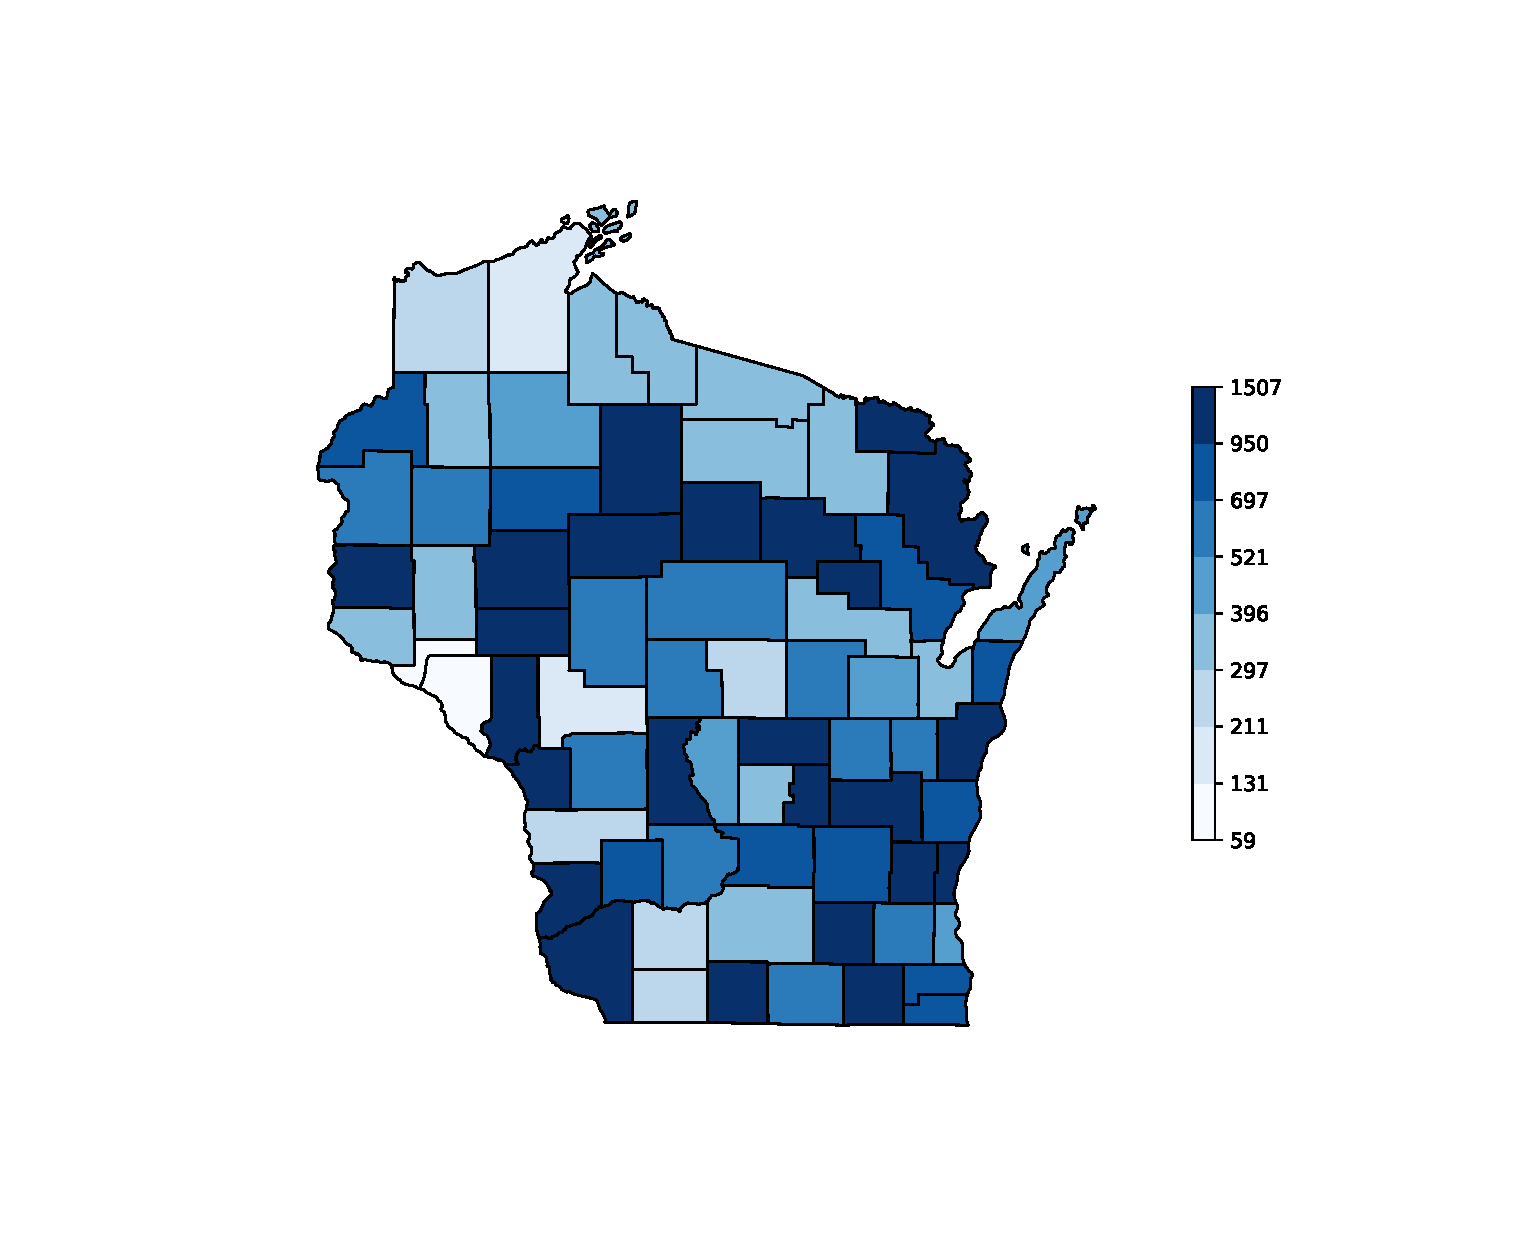
\includegraphics[width=.95\textwidth]{d5_ipw_1997.eps}
%\caption{5-Year Change in Imports per Worker 1997-2002 (US\$)}
%\label{fig:d5ipw}
%\end{center}
%\end{figure}
%
%\begin{figure}
%\begin{center}
%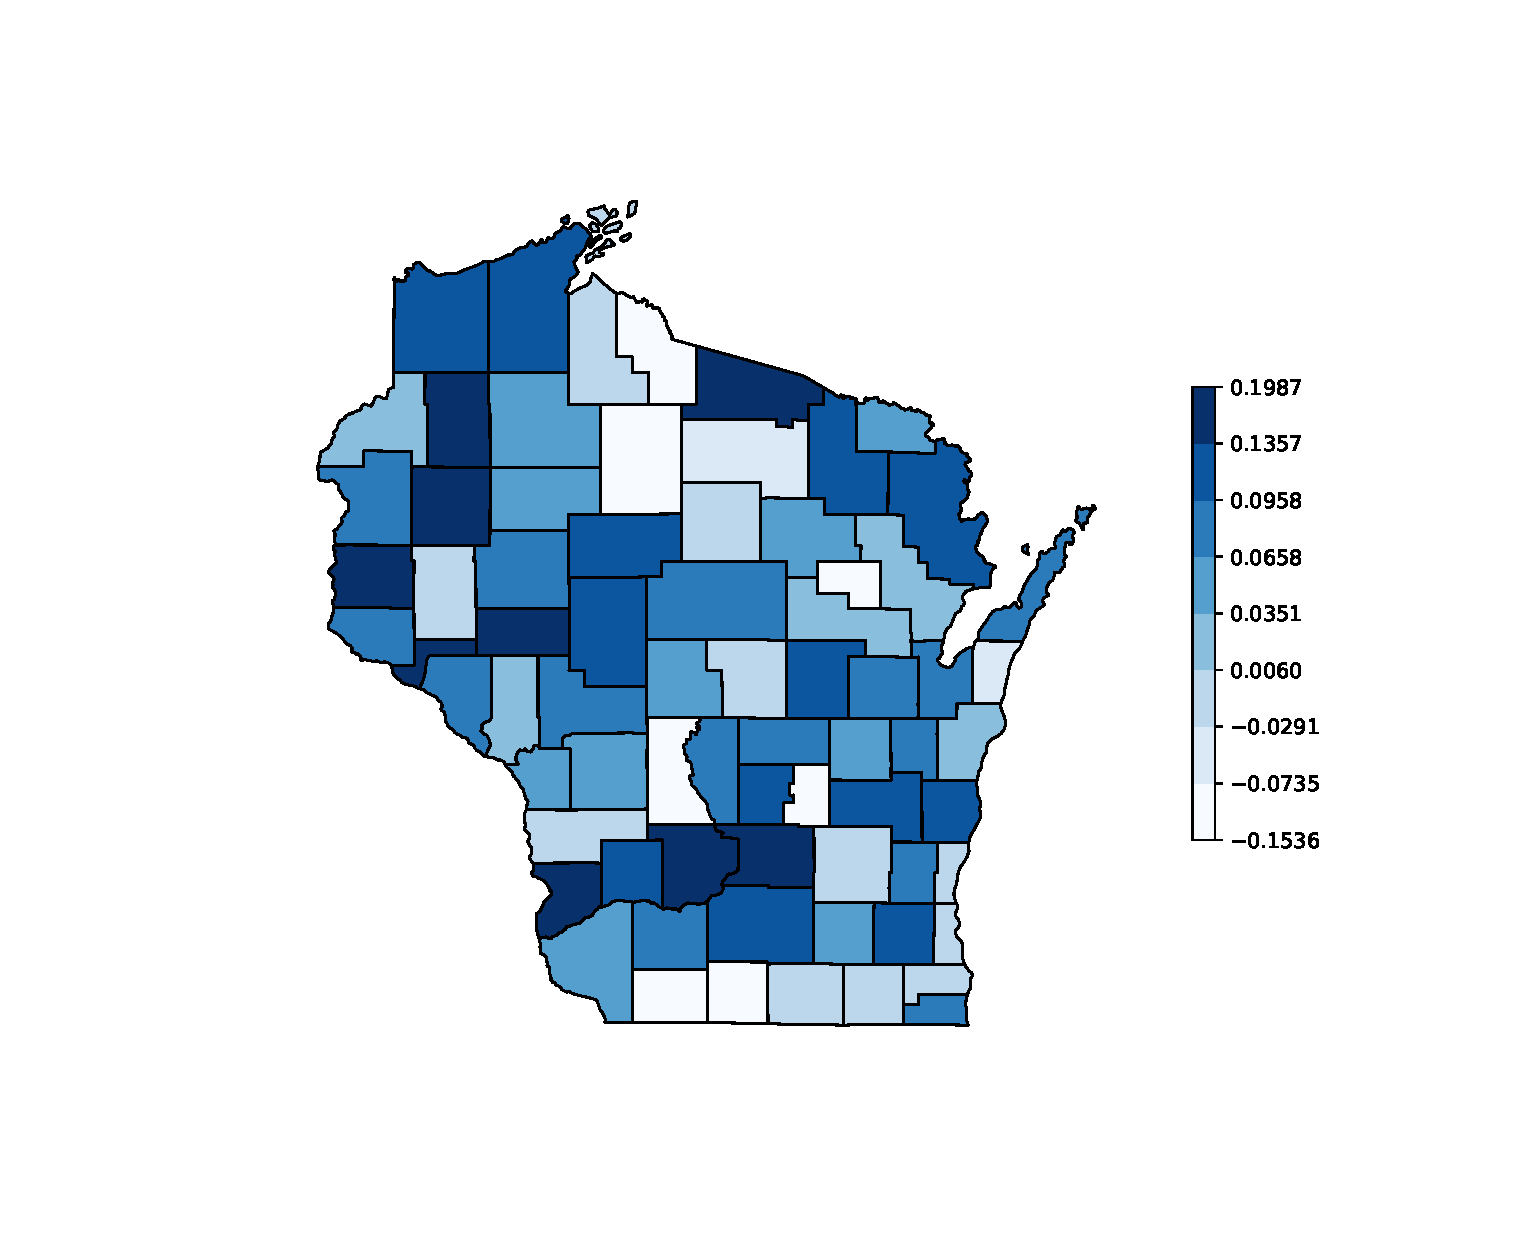
\includegraphics[width=.95\textwidth]{d5log_emp_i_97_02-1.eps}
%\caption{5-Year Employment Change 1997-2002 (Percent)}
%\label{fig:d5emp}
%\end{center}
%\end{figure}
%Maps for 1992-1997, 2002-2007, 2007-2011, and 2011-2016 (not included here) illustrate the same lack of relationship between imports and employment growth. This visual impression is also borne out statistically.
%
%The same regression as in column (5) of Table \ref{tab:2sls} with data for Wisconsin counties only yields similar coefficient estimates as the full national sample. The effect of the rise in manufacturing imports is somewhat stronger and significant at the 10 percent level, while the local share of employment in manufacturing is no longer statistically significant. The effect of local industry concentration, on the other hand, is stronger (-0.242 compared to -0.183 in the national sample) and remains statistically significant at the 5 percent level, suggesting that diversification at the county level plays an important role even in a state with a high proportion of manufacturing jobs compared to the national average.
%
%One plausible explanation that was not explored here is that the loss of manufacturing jobs was offset by job growth in the service sector. Nationally, \cite{Bloom:2019} find that this occurred particularly in local labor markets with a skilled workforce and, at a more granular level, that large multinational firms played a crucial role in this process. Due to data limitations associated with County Business Patterns, a more detailed analysis along these lines was beyond the scope of this paper but is an area for future research and certainly of interest from a policy perspective.
%\begin{figure*}[t!]
%    \centering
%    \begin{subfigure}[t]{0.5\textwidth}
%        \centering
%       
%        
%    \end{subfigure}%
%    ~ 
%    \begin{subfigure}[t]{0.5\textwidth}
%        \centering
%        
%    \end{subfigure}
%    \caption{W}
%\end{figure*}

\newpage
\bibliography{/Users/simeonalder/Dropbox/Bibliography/MasterBibliography}
\bibliographystyle{ecta}
\end{document}